\model{Deck of Cards}

There are 52 cards in a standard deck.
Each card has one of \emph{13 ranks} (1=Ace, 2, 3, 4, 5, 6, 7, 8, 9, 10, 11=Jack, 12=Queen, and 13=King) and one of \emph{4 suits} (0=Clubs, 3=Spades, 2=Hearts, and 1=Diamonds).
For example, ~\java{new Card(12, 2)} would construct the Queen of Hearts.

\vspace{1em}

The following deck is represented by an array of \java{Card} objects.
The array is one-dimensional, but the cards are shown in four rows (because of the paper margins).

\begin{center}
% http://www.milefoot.com/math/discrete/counting/cardfreq.htm
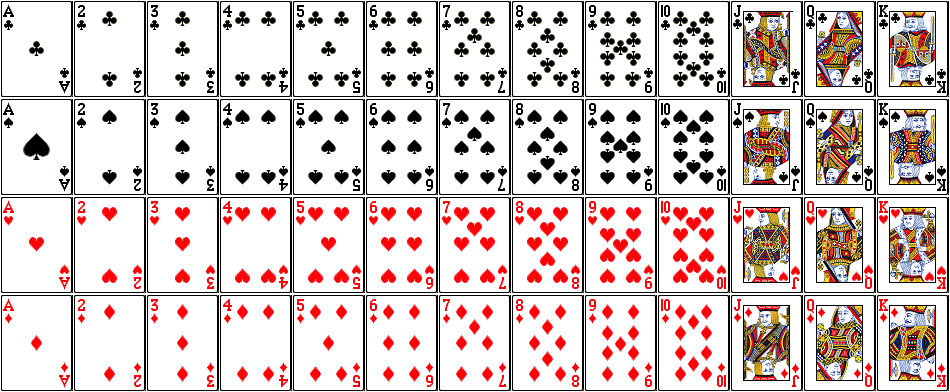
\includegraphics[width=\linewidth]{playing-cards1.png}
\end{center}


\quest{25 min}


\Q What is the index (in the array above) of the following cards?

\setlength{\defaultwidth}{3em}

\begin{multicols}{2}
\begin{enumerate}
\item Ace of Clubs     \ans{0}
\item Jack of Clubs    \ans{10}
\item 2 of Spades      \ans{14}
\item Queen of Spades  \ans{24}
\item 7 of Hearts      \ans{32}
\item King of Diamonds \ans{51}
\end{enumerate}
\end{multicols}


\Q Write the following statements using one line of code each.

\begin{enumerate}

\item Declare and initialize a \java{Card} array named \java{deck} that can hold 52 cards.
\begin{answer}[1em]
\begin{javaans}
Card[] deck = new Card[52];
\end{javaans}
\end{answer}

\item Construct the Ace of Clubs, and assign it as the first element in \java{deck}.
\begin{answer}[1em]
\begin{javaans}
deck[0] = new Card(1, 0);
\end{javaans}
\end{answer}

\item Construct the King of Diamonds, and assign it as the last element in \java{deck}.
\begin{answer}[1em]
\begin{javaans}
deck[51] = new Card(13, 1);    // or deck[deck.length - 1]
\end{javaans}
\end{answer}

\end{enumerate}


\Q Describe how you could repeat code from the previous question to construct the entire deck of cards (without having to type 52 statements).

\begin{answer}[3em]
Use nested for loops to iterate each possible \java{rank} and \java{suit}, construct that card, and assign it to the next index in the \jans{deck} array.
\end{answer}


\Q \label{build}
Discuss the following code as a team:

\begin{javalst}
int index = 0;
int[] suits = {0, 3, 2, 1};
for (int suit : suits) {
    for (int rank = 1; rank <= 13; rank++) {
        deck[index] = new Card(rank, suit);
        index++;
    }
}
\end{javalst}

\vspace{-1ex}
\begin{enumerate}

\item What is the overall purpose of the code?
\begin{answer}[1em]
It creates a deck of cards in the order shown in \ref{\currfilename}.
\end{answer}

\item Why is the \java{suits} array not just \{0, 1, 2, 3\}? (See \ref{\currfilename}.)
\begin{answer}[1em]
Because the picture shows the suits in a different order.
\end{answer}

\item Why does the code use an enhanced for loop for \java{suit}?
\begin{answer}[1em]
The code iterates the suits out of order, as specified in the array.
\end{answer}

\item Why does the code use a standard for loop for \java{rank}?
\begin{answer}[1em]
The code iterates the ranks in order; no array is needed for that.
\end{answer}

\item What is the purpose of the \java{index} variable?
\begin{answer}[1em]
To keep track of where to store the next card (not based on rank and suit).
\end{answer}

\end{enumerate}
\vspace{-1ex}


\Q \label{search}
Write a method named \java{inDeck} that takes a \java{Card[]} representing a deck of cards and a \java{Card} object representing a single card, and that returns \java{true} if the card is somewhere in the deck.
%Be sure to use the equals method of the \java{Card} object to make comparisons.
%Your solution must avoid \java{NullPointerException} if any cards are missing.
%(Hint: Start with your solution to \ref{foreach}.)

\begin{answer}[10em]
\begin{javaans}
public static boolean inDeck(Card[] deck, Card card) {
    for (Card c : deck) {
        if (c != null && c.equals(card)) {
            return true;
        }
    }
    return false;
}
\end{javaans}
\end{answer}


\Q \label{sort}
 Describe what the following code does and how it works.
(Note: You've come a long way this semester, to be able to understand this example!)

\begin{javalst}
public static Card[] sort(Card[] deck) {
    if (deck == null) {
        System.err.println("Missing deck!");
        return null;
    }
    Card[] sorted = new Card[deck.length];
    for (Card card : deck) {
        int index = card.position();  // returns suit * 13 + rank - 1
        sorted[index] = card;
    }
    return sorted;
}
\end{javalst}

\vspace{-1ex}
\begin{enumerate}

\item What is the overall purpose of the code?
\begin{answer}[1em]
This example sorts an array of cards.
\end{answer}

\item What is the purpose of the if statement?
\begin{answer}[1em]
It avoids \java{NullPointerException} if \java{deck} is invalid.
\end{answer}

\item Does this method modify the \java{deck} array? Justify your answer.
\begin{answer}[1em]
No; it creates and returns a new array named \java{sorted}.
\end{answer}

\item How does the \java{sort} method know where to put each card?
\begin{answer}[1em]
It computes the \java{position} based on its rank and suit.
\end{answer}

\end{enumerate}
\vspace{-1ex}


\Q Identify the following Java language features in the previous question.

\setlength{\defaultwidth}{15em}

\begin{minipage}{22.5em}
\begin{enumerate}

\item variables
\hfill \ans{deck, sorted, card, index}
\item decisions
\hfill \ans{if (deck == null)}
\item loops
\hfill \ans{for (Card card : deck)}
\item methods
\hfill \ans{sort, println, position}
\item arrays
\hfill \ans{deck, sorted}
\item objects
\hfill \ans{"Missing deck!", card}

\end{enumerate}
\end{minipage}
